\documentclass[]{article}
\usepackage{fullpage}
\usepackage[authoryear]{natbib}
\usepackage{setspace}
    \doublespacing
\usepackage{hyperref}
\hypersetup{
    colorlinks,
    citecolor=black,
    filecolor=black,
    linkcolor=cyan,
    urlcolor=cyan
}
\usepackage{amssymb,amsmath}
\usepackage{bm}
\usepackage{dcolumn}
\usepackage{booktabs}
\usepackage{url}
\usepackage{tikz}
\usepackage{todonotes}
\usepackage[utf8]{inputenc}
\usepackage{graphicx}
\usepackage{longtable}
\usepackage{todonotes}
\usepackage{lscape}
\usepackage{float}


\title{Measuring Real-time Perceptions of Financial Market Stress}
\author{Christopher Gandrud and Mark Hallerberg \\ \emph{Hertie School of Governance}\footnote{Please contact Christopher Gandrud
(\href{mailto:gandrud@hertie-school.org}{\nolinkurl{gandrud@hertie-school.org}}).
Thank you to Ronen Palan for helpful comments, as well as Christian Franz and Sahil Deo for early research assistance. Our research is generously supported by the Deutsche Forschungsgemeinschaft. All data and replication material can be found at:
\url{https://github.com/christophergandrud/EIUCrisesMeasure}.}}

\begin{document}

\maketitle


\textbf{Incomplete Working Draft}

\begin{abstract}
Research into the causes, responses to, and effects of banking crisis needs a measure of banking crises that is: accurate, reliable, comparable across countries, and ideally includes information about crisis severity. Most work to-date uses one of two series of crisis data: \cite{Reinhart2009,ReinhartRog2010} or \cite{laeven2013} and its predecessors. These measures are lacking in that they are constructed post-hoc and so tend to be biased towards severe crises and away from circumstances where governments effectively calmed emerging trouble. This creates clear selection bias. In addition, they are simple dichotomous indicators of financial crisis and do so do not indicate crisis severity. We use a kernel principal component analysis (PCA) of Economist Intelligence Unit monthly country reports to develop a new real-time and continuous measure of perceived banking system stress. We refer to this measure as the EIU Perceptions of Financial Market Stress (EPFMS) Index. We not only develop a novel indicator of financial market stress, but also make a contribution to the wider political science and finance literatures on measurement by demonstrating how kernel PCA can be used to summarize vast quantities of qualitative texts into useful cross-sectional time-series indicators.
\end{abstract}

Why and how do politicians respond to financial market stress? What are the political consequences of crises? These questions have attracted considerable attention following the
2007-2009 crisis, and earlier late-1990s Asian financial crisis. However, almost all research on these topics lack a crucial variable: a real-time indication of the level of financial
market stress that policy-makers perceived. To understand why politicians made a given choice in response to financial market stress, we need to have a measure of the conditions that they believed they were responding to. Most recent research on the political responses to and effects of financial crises has relied on second-best alternatives; either one of two measures of financial crisis--\cite{Reinhart2009,ReinhartRog2010} or \cite{laeven2013} and its predecessors. These measures are post-hoc binary assessments of crisis occurrence and therefore are particularly lacking for studying politicians actions in response to financial crisis.

In this paper we aim to develop a new index
of real-time perceptions of financial market stress. The Index is
created using a kernel principal component analysis (PCA) of detailed qualitative data, namely monthly Economist Intelligence Unit (EIU) reports. We call it the EIU Perceptions of
Financial Market Stress (EPFMS) Index. This measure should be used instead of
previous second-best measures of financial market stress by researchers
aiming to understand why and how policy-makers respond to financial
crisis. In so doing, we also make a contribution to the wider political
science literature by showing how kernel PCA can be used to summarize
vast quantities of qualitative texts into cross-sectional time-series
indicators.

We start the paper by detailing previous attempts to measure financial market crises and stress and areas where they could be improved. We then discuss the
construction of the EPFMS Index and undertake a number of approaches to assessing its validity. This includes, comparing it to widely used previous measures of financial market stress that are based on both quantitative and qualitative data. We then further explore important characteristics of the Index including how it differs across developed and developing countries and how it changes over time within countries. Doing so allows us to draw conclusions about how financial market conditions differ across countries and how perceptions of financial market stress change over the course of a crisis.

\todo{Plan to include at least one replication.}

\section{Motivation}\label{motivation}

Knowing when crises started, when they ended, and how severe they were over their course is crucial for research trying to understand how governments choose to respond to financial market distress, the fiscal costs of these responses, and the political outcomes. Researchers working on these issues have tended to rely on two data sources of cross-country information on when a country is facing a financial crisis--\cite{Reinhart2009,ReinhartRog2010} or \cite{laeven2013} and its predecessor versions. For a literature review see \cite{GandrudHallerberg2015}, as well as tables \ref{LitRevTable} and \ref{LitRevTable2} in the Online Appendix.

There are a number of problems with these indicators. Chiefly, crises are identified \emph{post hoc} by researchers who know what happened after the fact. Financial market stress that is addressed well by policymakers, thus preventing a major crisis, may therefore not be included. Similarly, stress that is temporarily dampened through unsustainable policy measures, only to flare up later, is not clearly recorded. This makes it difficult to adequately study why and how politicians respond to financial market stress.

The measures are dichotomous. So, they do not give any indication of how
severe a crisis was. Having a dichotomous measure also means that measurement errors--incorrectly timing the start or end of a crisis--can have large consequences for creating bias in econometric models where they are used. Measurement error is a significant problem in this data. Unlike economic recessions, financial crises are poorly defined in previous sources. There are large inconsistencies between the timing of crises in the \cite{laeven2013} and \cite{Reinhart2009} data sets \citep{Chaudron2014}. For example, Japan is labeled as having a crisis between 1997 and 2001 by the former, but 1992-1997 in the latter. \cite{GandrudHallerberg2015} find that there are significant difference in crisis timing between different versions of the \cite{laeven2013} data. The measures are at gross intervals, typically yearly, prohibiting sub-annual analysis. Finally, while the measures use fairly precise definitions of when a crisis started (see Table \ref{comp_table} for a summary), reasons for dating the end of a crisis are either unstated as in the case of \cite{Reinhart2009} or ad hoc. Laeven and Valencia \citeyearpar[footnote 19]{laeven2013} determine that a crisis has concluded when real GDP and real credit growth are positive for two years, or five years after the crisis began.

Overall, we lack a continuous real-time measure of financial market stress that we need to be able to adequately examine why and how policy-makers respond to financial market problems.

\begin{table}
    \caption{Comparision of Crisis Measures' Definitions}
    \label{comp_table}
    \begin{center}
        \begin{tabular}{m{3cm} | m{2cm} m{2cm} m{7cm}}
            Source & Measurement Level & Periodicity &  Definition of Financial Market Distress/Crisis \\
            \hline\hline
                Reinhart and Rogoff \citeyearpar[11]{Reinhart2009,ReinhartRog2010} & binary & annual & One of two types of events: (1) bank runs leading to closures, mergers, or public sector takeovers of one or more financial institution or (2) the closure, merger, takeover, or large-scale government assistant of an important financial institution marking the start of a string of similar events.  \\
                Laeven and Valencia \citeyearpar[228]{laeven2013} & binary & annual & Meets two conditions: (1) significant sign of financial distress in the banking system and (2) significant banking policy intervention measures in response to significant losses in the banking system.  \\
                Romer and Romer \citeyearpar[3]{Romer2015} & ordinal (0 to 15 scale) & bi-annual & Hand-coded perceptions of funding problems and rising loan defaults in \emph{OECD Economic Outlook}  \\
            \hline
        \end{tabular}
    \end{center}
\end{table}

\cite{Romer2015} attempted to solve many of the problems in the \cite{Reinhart2009} and \cite{laeven2013} data sets by manually
classifying 24 countries on a 16 point scale of the cost of
credit intermediation. They code countries using information from OECD
semi-annual \emph{Economic Outlook} reports from 1967 to 2007. Relying
on contemporaneous reports allows for the construction of a real-time
measure of credit market distress. This would allow us to examine policy
choices that head off trouble or unsustainably prolong brewing
difficulties. Their, relatively, continuous measure gives an indication
of market distress intensity.

Their approach is limited in a number of key ways. First, they
are necessarily confined to the relatively small sample of OECD
countries. Second, their measure is laborious to create and update. If there was a more encompassing corpus of texts than the OECD \emph{Economic Outlook}, actually applying the method would be very costly. Third, relying on human coders introduces well-known problems of inter-coder reliability.

Others have attempted to create measures of national banking system fragility and crisis using using quantitative accounting and economic data. The finance literature widely uses a statistical quantity know as `Z-Scores', originally developed to assess firm solvency \cite{roy1952}, to measure national financial system fragility when examining how banking system structure and policies affect the probability of bank-specific and financial system difficulties \citep[e.g.][]{beck2013bank,vcihak2010islamic,laeven2009bank,uhde2009}. Though there are various ways to calculate this measure \citep[73]{Lepetit2013}, in general uses bank accounting information--assets, equity, and return on assets--to create an inverse measure the probability of a country's `banking system insolvency'.

Another approach to measuring crises, though not necessarily crises confined to the banking sector, is to classify periods below a pre-specified output gap. For example, in his examination of reforms in response to economic crises, including financial crises, Galasso determines a crisis to be when the output gap falls below the 90 percentile in his sample \citeyearpar[154]{galasso2014}. Other work, notably \cite{laeven2013} and \cite{Reinhart2009} examine the output gap as a consequence of crisis, rather than the crisis itself.

There have been a number of recent innovations to measuring banking system stability using quantitative data. Building on \cite{vonHagen2007}, \cite{Jing2015} developed an index of money market pressure based on changes in short-term interest rates and stocks of central bank reserves. However, this measure conflates distress and policy responses, assuming central banks use the same reaction function to increased demand for liquidity. \cite{Rosas2009} developed a dynamic latent trait model of banking system distress. His measure relies on nationally reported data to the IMF's International Financial Statistics (IFS). \cite{GandrudCopHal2015} show that data reporting to the IFS is very uneven across countries and time. They indicate that decisions to report data to the IFS could be endogenous to political events, complicating attempts to use IFS data to date crisis occurrence and severity. Furthermore, as \cite{KayserLeininger2015} show, people make decisions based contemporaneously available data, but researchers often use data that has been updated after the fact. Using revised IFS data will give an inaccurate impression of the conditions that politicians believed they were in at the time. Apart from Z-Scores, one version of which is available from the World Bank's Global Financial Development Database \citep{worldbank2013}, these various quantitative measures have not been made publicly available to researchers.

\section{~Creating the EIU Perceptions of Financial Market Stress
Index}\label{creating-the-perceptions-of-financial-market-stress-index}

We overcome many of the problems that plague previous measures by using a new approach to estimating real-time perceptions of financial market stress. Our method uses kernel principle component analysis \citep{Scholkopf1998,lodhi2002,Spirling2012} of country reports from the \emph{Economist Intelligence Unit}\footnote{See \url{http://www.eiu.com/}. Accessed May 2015.} to create a monthly index for almost all countries from 2003 through 2011.

\subsection{Why the EIU?}\label{why-the-eiu}

The EIU is the compilation of real-time, third-party
assessments of financial market conditions reported monthly or, for a subset of countries, quarterly. These reports contain both summaries of
present and future economic conditions. They are also a channel through which this information is disseminated to public and private actors. Together, the reports create a very large corpus
(more than 20,000 texts from 1997 through 2011) of
reports for more than 100 countries. As the texts generally follow the
same format and style, they contain directly comparable assessments of
economic conditions across the globe for a significant time
span. In contrast, the OECD \emph{Economic Outlook} provides comparable
reports for a very small number of wealthy countries on a bi-annual
basis. As such, the EIU is preferable for creating a cross-country indicator of perceived financial market stress.

\subsection{Summarizing Financial Market Stress in the
EIU}\label{summarizing-financial-market-stress-in-the-eiu}

Our aim is to create an index that classifies financial conditions on a
continuous more-stressed/less-stressed spectrum for as many country-months as possible. Therefore, we clearly need an efficient way to summarize the vast quantity of information in the EIU reports along such a spectrum. To do this we first collected and processed the texts. We then used kernel principal component analysis to summarize the texts into a
dimension of financial market stress. We rescaled the Index to ease
interpretation.

\subsubsection{Text selection}\label{text-selection}

EIU reports assess many economic sectors within a country,
not just the financial sector. So, our first step was to select the
portions of the EIU texts that contained relevant information about
countries' financial systems. We automatically collected and the parsed
reports--the reports were in HTML format. We then extracted the portions
of the texts--headlines and paragraphs--that contained at least one of a
number of keywords concerning financial markets.\footnote{The
  keywords included: \emph{bail-out}, \emph{bailout}, \emph{balance
  sheet}, \emph{balance-sheet}, \emph{bank}, \emph{banks},
  \emph{banking}, \emph{credit}, \emph{crunch}, \emph{default},
  \emph{finance}, \emph{financial}, \emph{lend}, \emph{loan},
  \emph{squeeze} {[}MAKE SURE TO UPDATE{]}. These keywords were adapted
  from those used by \cite{Romer2015} and are intended to
  select passages that discuss credit market conditions.} Due to a
significant change in how the reports were constructed in 2003, we also
selected only texts from 2003 in order to maintain comparability across
the time-series.

We then preprocessed these texts using standard techniques \citep[see][]{Grimmer2013}.\footnote{All preprocessing was done using the \texttt{tm} package \citep{tm2015} in R \citep{R-cite}.} This involved removing common English words, such as `was' and `its'. The `stopword' list we used was from \cite{dhillon:modha:mlj01}. We stemmed the words so that different variants of the same word are grouped together. We removed extra whitespace between the words, as well as removed punctuation and numbers. Finally, we dropped texts that included very few words (less than six). In practice, including these texts had prevented the estimation of the kernel PCA model.

\subsubsection{Kernel Principal Component
Analysis}\label{kernel-principal-component-analysis}

Texts are frequently summarized using unordered `bags-of-words'
approaches, such as Latent Dirichlet Allocation, that do not retain word
order. The result of these approaches is often clusters (bags) of `topics'
within speeches or clusters of speeches around topics \citep[for a review see][]{Grimmer2013}. We would like to accomplish something different. Ideally,
we would like to preserve the order of the words in our texts and we
would like to place the texts on a continuous scale that will be
interpretable as a measure of perceived financial market stress. We
would like to preserve the order of the words in the texts. Many
financial terms such as `credit growth' and `borrowing costs' are used
in completely different senses depending on the adjectives that modify
them. For example, `slowing credit growth' vs. `expanding credit growth'
or `falling borrowing costs' vs. `increasing borrowing costs'. Likewise, adjectives can have very different implications for describing market conditions depending on the nouns that they modify. For example, `increasing' can indicate worsening conditions as in `increasing non-perfomring loans' or improving conditions as in `increasing lending'.  A
bags-of-words approach that treated each word as having meaning as an
individual unit, rather than having meaning in ordered association with
other words, would not adequately capture common and radically different
meanings in the EIU documents.

In order to address these issues we use kernel principal component
analysis. This method was developed by \cite{Scholkopf1998} and \cite{lodhi2002}. \cite{Spirling2012} introduced it into political science. He used it to summarize changing
  trends in treaties between the US government and Native American
  groups. Kernel PCA allows us to extract structure from our likely
high-dimensional EIU corpus (Zhang, Wang, and Ma 2010, 6531--37) while
preserving word order.

Our unit of analysis is a sub-string kernel: in
effect a short sequence of letters\footnote{Following \cite{Spirling2012},
  we used kernels with a length of five, i.e.~those that are five letters
  long. See also \cite{lodhi2002} who demonstrate that in English
  string lengths between four and seven are often optimal.} that can be
shared within and across words. Thus we can distinguish between two
simple documents with the stemmed strings `slow credit' and `expand
credit'. They share the five character kernels `credit, but differ on
`slowc' and `pandc' among others. Using \cite{lodhi2002} we can
summarize the similarity of these documents with the frequency
distribution of five-length strings that they have in
common--i.e. one--standardized by document length. We can find these pairs
for all of the documents in our corpus to create a kernel matrix.
Finally, we can scale the documents using principal component
analysis.\footnote{We conducted kernel PCA with the \texttt{kpca}
  function from the R package \textbf{kernlab} (Karatzoglou et al.
  2004).}

\subsubsection{Dimensionality}\label{dimensionality}

To determine the number of dimensions that best describe the data, we
conducted a scree test, the results of which are shown in Figure
\ref{scree_plot}. There is something of an `elbow' in the plot at three components.
This suggests that there is perhaps substantively meaningful variation in
approximately the first three dimensions. The drop from the first to
second component is notable. In the rest of the article we focus on the first dimension as the main dimension summarizing financial market conditions. We also examined a number of the other dimensions. However, these noticeably did not closely correspond to our priors about financial market stress based on previous indicators.

\begin{figure}
    \caption{Assessing Model Fit: Eigenvalues for Kernel Principal Components}
    \label{scree_plot}
    \begin{center}
        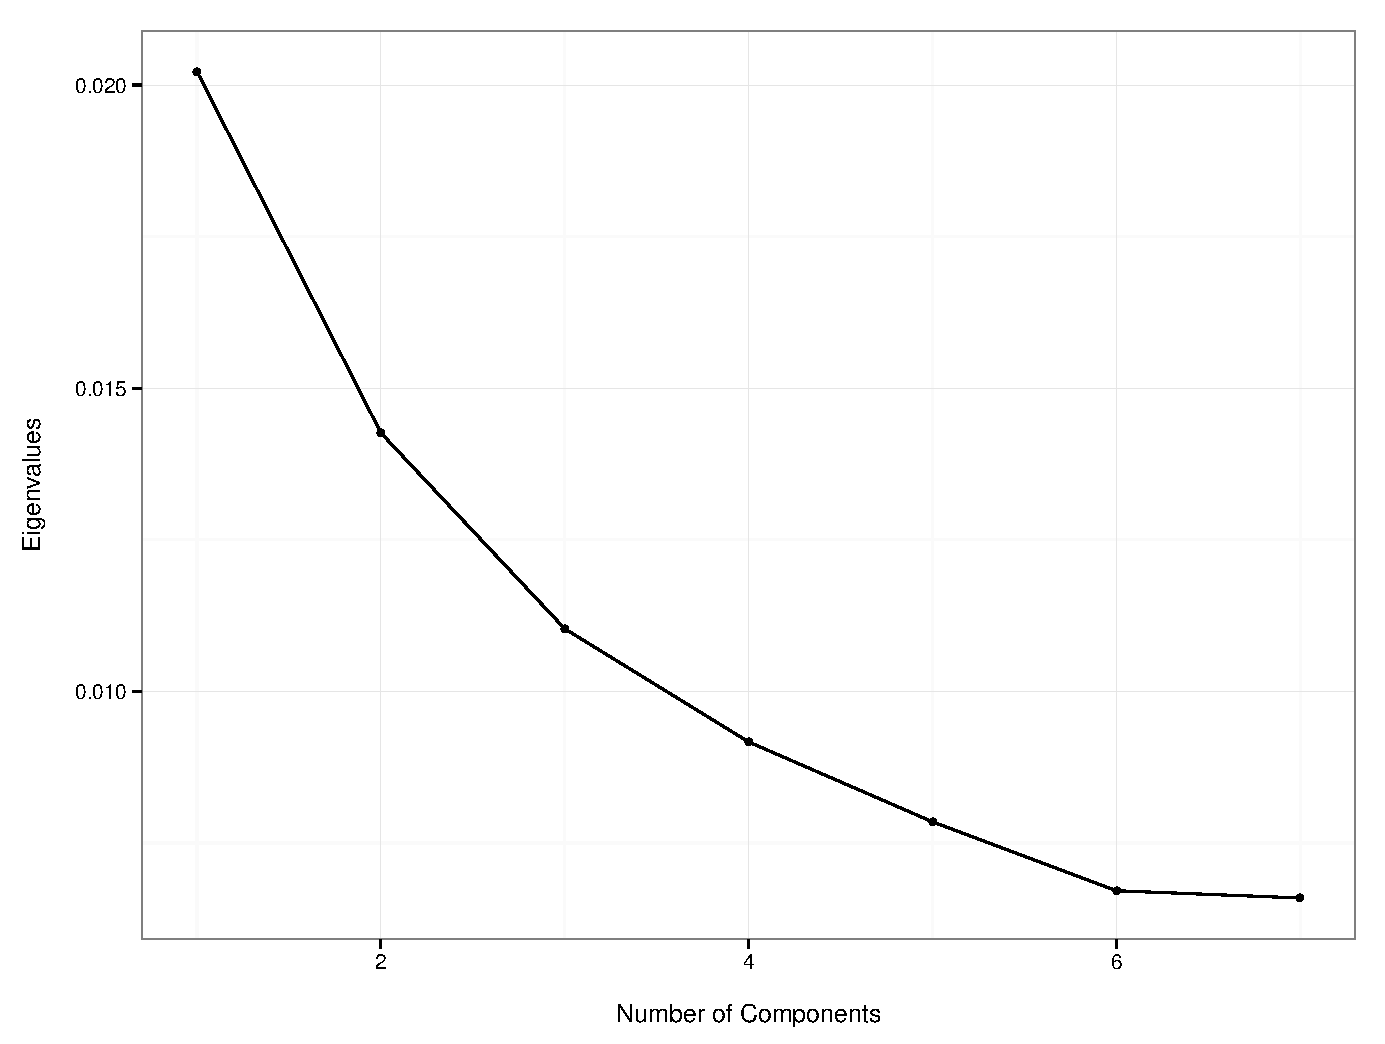
\includegraphics[scale=0.5]{analysis/figures/scree_plot.pdf}
    \end{center}
\end{figure}

\section{Results, Validation, and Description}\label{results}

The lines in figures \ref{compare_1} and \ref{compare_2} show the
results of the kernel PCA analysis--the first principal compenent--for a selection of countries. Similar plots for all countries in the analysis are available in the Appendix. Before diving deeper into these results, it is important to note three simple transformations we conducted on the raw results. First, we flipped the
scale. As we demonstrate when we compare the Index to other measures of
crisis, this allows higher values of the EPFMS to be interpreted as
`more financial market stress'. Second, we rescaled the Index so that it
would be between zero and one.\footnote{\(\frac{x - \mathrm{min}(\bm{X})}{\mathrm{max}(\bm{X}) - \mathrm{min}(\bm{X})}\),
  where \(\bm{X}\) is the vector of the first principal component and
  \(x\) is an individual value from this vector.} This eases
interpretation and comparability to other measures. Henceforth we only
use the rescaled version of the Index. Then we slightly smoothed the
results by taking a two period--usually two months--moving average.

What does this dimension represent? We took a number of approaches to
answer this question. First, following \cite{Spirling2012} we used a random
forests regression \citep{Breiman2001,jones2015} to examine the
relationships between word stems from the texts and the Perceptions
Index. Second, we compared the Index to previous indices using an
`interocular' test, i.e. looking at plots of the results and comparing
them to our priors on financial market stress.

\subsection{Random forests and Correlations}\label{random-forests}

Spirling \citeyearpar[6--8]{Spirling2012} demonstrated the usefulness of using random forests
``regressions'' to explore what principal components from textual
analyses represent. To use this tool to explore our data, we first created a document-term
frequency matrix from the stemmed documents. Effectively this is a
\(k \times s\) matrix recording the frequency of each term in \(\bm{S}\)
for each document in \(\bm{K}\). We removed sparse terms, i.e.~kept only
stems that were found in 90 percent of the documents. Random forests
regressions, as opposed to ordinary least squares regressions, are useful
for exploring this data's associations with the estimated principal components because it can handle many variables--in this case 958 stems--relative to the number of documents--12,473.

We focus on the variable importance from this analysis.\footnote{We conducted the random forests regressions using the \texttt{rfsrc} function from the
\textbf{randomForestSRC} R package \citep{randomForestSRCCite}.} The results are shown in Figure \ref{rf_importance}. The logic behind variable importance in this context is as a measure of how well the frequency of a given stem in a text allows the model to predict the EPFMS score for that text.

Unsurprisingly, two of the three stems with the largest variable importance are `bank', `financi', and `loan'. Terms with these stems were used to select the texts. The prevalence of these terms and others that are clearly related to the financial sector, such as interest, rate, and fund, indicate that the EPFMS is indeed about financial sector conditions and not some other topic.

\begin{figure}
    \caption{40 Stems Estimated to be the Most Important for Predicting EIU Perception of Financial Market Stress Index}
    \label{rf_importance}

    \begin{center}
        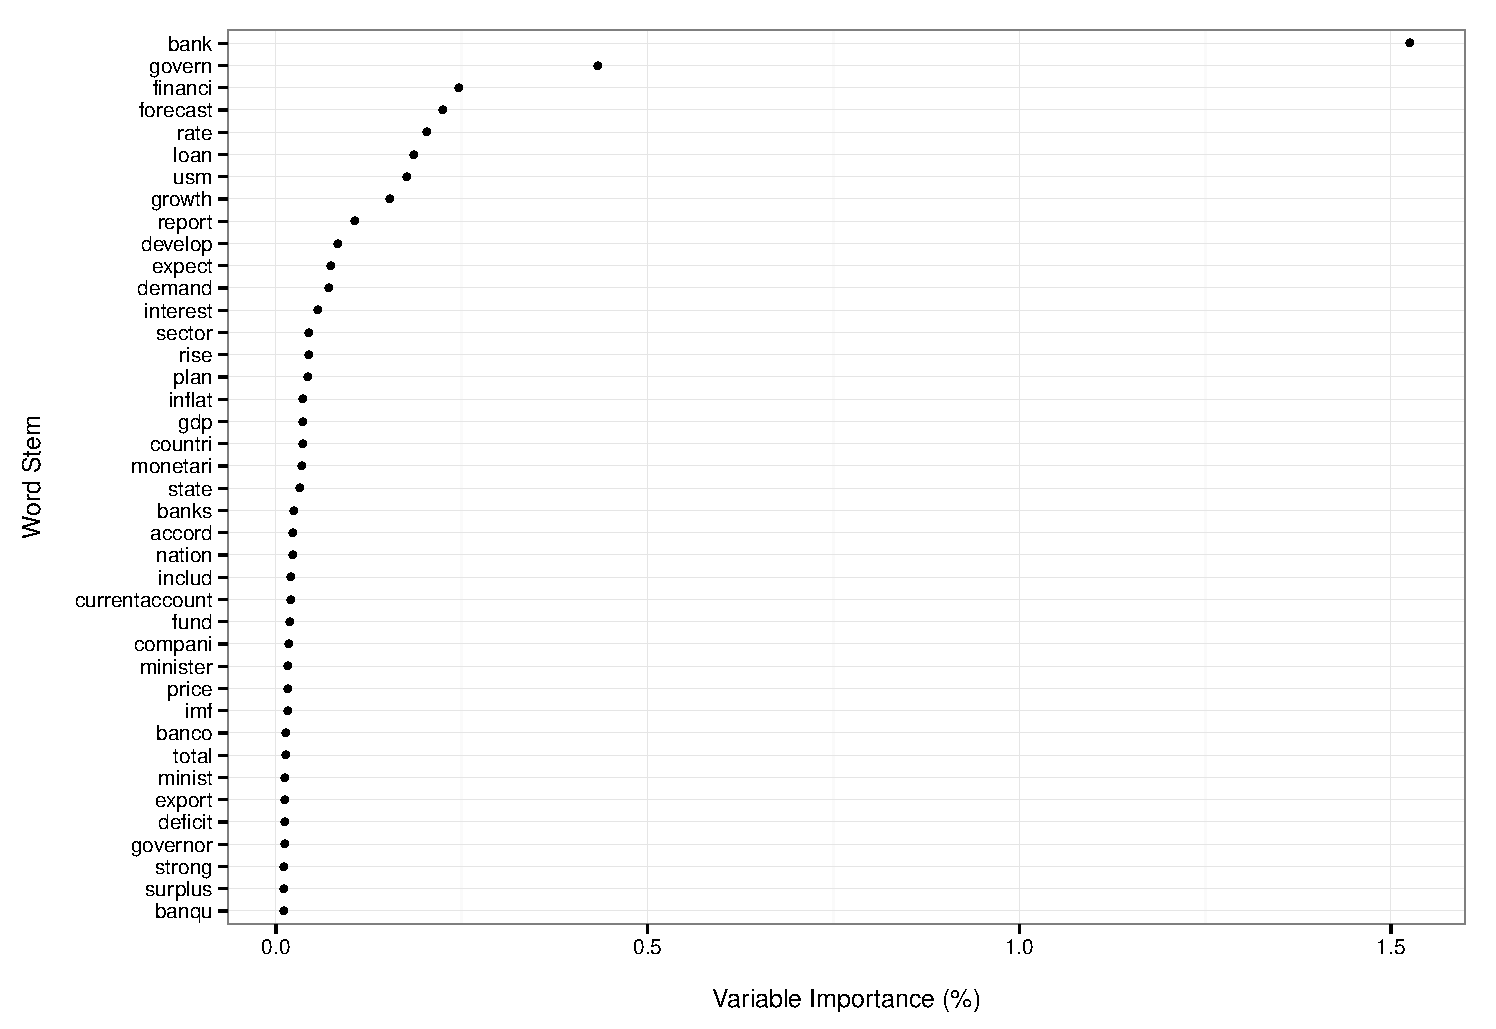
\includegraphics[scale=0.5]{analysis/figures/rf_stem_importance.pdf}
    \end{center}

\end{figure}

\subsection{Comparison to other crisis
measures}\label{comparison-to-other-crisis-measures}

How does our measure compare to previous ways of measuring and timing
financial market stress and crisis? We directly compare our measure to
dichotomous measures in \cite{Reinhart2009} and \cite{laeven2013}, as well as Romer and Romer's (2015) continuous measure.

There are some limitations in comparability based simply on the
different coverage of the different indices. \cite{Romer2015}
in particular largely does not include the most recent crisis in their
sample as they did not collect data past 2007. We had to make a number
of transformations and assumptions to be able to compare the different
data sets. First, the Laeven and Valencia and Reinhart and Rogoff data
on recorded only at yearly intervals. So, we assumed that the crisis
start and end dates they referred to were in the middle of the year,
i.e. June. Second, we rescaled Romer and Romer's 16-point scale (in effect 14-points because they do not classify any country-quarter in
their sample as being at the upper two positions on the scale) to be
between 0 and 1 using the same method as above. Finally, it should be
noted that \cite{Reinhart2009} only cover 70 countries and they
have updated their data least recently.

The solid lines in figures \ref{compare_1} and \ref{compare_2} show the
EIU Perceptions of Financial Market Stress Index. The dashed lines show
Romer and Romer's (rescaled) measure. Finally, the shaded boxes show the
periods where \cite{laeven2013} and \cite{Reinhart2009} classify there as being a banking crisis.\footnote{We used Table 1 in \cite{Romer2015} to recreate their data set. We downloaded Laeven and Valencia's data from: \url{https://www.imf.org/external/pubs/cat/longres.aspx?sk=26015.0}.
  Accessed May 2015. Reinhart and Rogoff's data was downloaded from:
  \url{http://www.carmenreinhart.com/data/browse-by-topic/topics/7/}.
  Accessed May 2015.} It should be noted that \cite{laeven2013} identify eight ``borderline'' crises in this period, in that the countries almost meet their systemic banking crisis definition because they only used two rather than three policy responses.\footnote{The cases are: France, Hungary, Italy, Portugal, Russia, Slovenia, Sweden, and Switzerland.} Some of these borderline cases are shown in the figures \ref{compare_1} and \ref{compare_2}.

In many cases--given the time period limitations of each data series--,
the indices overlap. Comparisons with \cite{Romer2015} are limited, but we can see that in general, where comparable time series are available, that the EPFMS and their index are roughly similar. In particular, both indices increase in the US from early 2007. They both decline for Japan through 2004-2005. A notable difference is
how Romer and Romer classify Japan as being without stress from
mid-2005, while the EPFMS stays high relative to many other economically
developed countries. While they both classify Iceland as being under
stress in the late 2000s, the timing is different. Romer and
Romer classify Iceland as in stress\footnote{They classify Iceland as
  being in a ``minor crisis'' in the second half of 2006 and a ``credit
  disruption'' in the first half of 2007.} in 2006-2007. This is earlier
than not only a marked increase in the EPFMS Index, but also Reinhart
and Rogoff and Laeven and Valencia's timing.

\cite{Reinhart2009} sometimes start dating a crisis before \cite{laeven2013}--particularly in Iceland and Ireland. This could reflect the slightly different definitions that they use. As summarized in Table \ref{comp_table}, \cite{Reinhart2009} date crises when bank runs occur. \cite{laeven2013} begin the crisis clock when not only are there significant events in the financial system, but also when the government follows the distress with a policy response.

One useful characteristic of the EPFMS is that we can use it to follow the
progression of crises over time. \cite[227]{laeven2013} comment
that part of the problem with dating financial crises is that they
develop differently:

\begin{quote}
    Some crises evolve gradually, gaining speed as the ripple effects from a seemingly small shock propagate forward in time \ldots other episodes happen more abruptly and are often the result of sudden stops.
\end{quote}

The real-time and relatively granular nature of the EPFMS allows to
distinguish these types of crises. For example, we can see in Figure
\ref{compare_2} that financial market difficulties in the United States
crisis built over along period of time, with a few spikes during notable
banking difficulties. Conversely, countries such as Germany, Hungary,
and Iceland clearly have much more sudden periods of perceived financial
distress. Using an binary definition of crises would no allow us to
capture these trajectories.

We can use the EPMFS to identify periods where financial market
conditions were perceived to be worsening, though for whatever reason
these perceptions changed before other measures would record a financial
crisis. Australia, Brazil, and the Czech Republic, among others, in
about late-2008/2009 are notable examples. They all see noticeable
spikes in perceptions of stress shortly after Lehman Brothers collapsed
in the US. Fairly quickly thereafter, their EPMFS scores return to
previous levels. Laeven and Valencia and Reinhart and Rogoff do not
record these episodes as crises. The perceived stress likely experienced
by policy-makers at this time would therefore be excluded from political
science work using previous binary measures of crisis.

The advantages of the EPFMS are also apparent for timing the end of financial crises. This is a particularly difficult issue for the binary indicators. Though crisis onset is typically well defined, these measures rarely have a clear or non-ad hoc way of determining when a crisis has ended. Though we are limited in the range of EIU texts we have at our disposal, it is clear that some countries, notably then United Kingdom and the United States, were perceived to be having improved financial market conditions from about 2010. Other countries, particularly in Western and Southern Europe plateaued at a high level through the end of 2011. While still others go through `double dips'. Italy, for example, appeared to be improving in late 2009 through mid-2010. But perceptions worsened around 2011, likely in relation to the Eurozone crisis. Laeven and Valencia's measure simply describes this entire period as a crisis. Not only does the EPMFS allow us to more accurately date when conditions were seen to have improved, but it also allows us to study this trajectory of these improvements.

Overall, the similarities between EPFMS scores and other measures of crises suggests that the EPFMS Index does capture aspects of financial market stress. In particular, higher values of the EPFMS are indicate higher levels of perceived financial market stress. At the same
time, the differences between the measures also indicates that the EPFMS
sheds unique light on processes not captured well by previous indices.
One major difference that we will now look at in more detail is how
having a continuous indicator allows us to consider how levels perceived
financial market stress differ between developed and developing
countries.

\begin{figure}
    \caption{Comparing Perceptions of Financial Market Conditions to \cite{laeven2013} and \cite{Reinhart2009} (1)}
    \label{compare_1}
    \begin{center}
        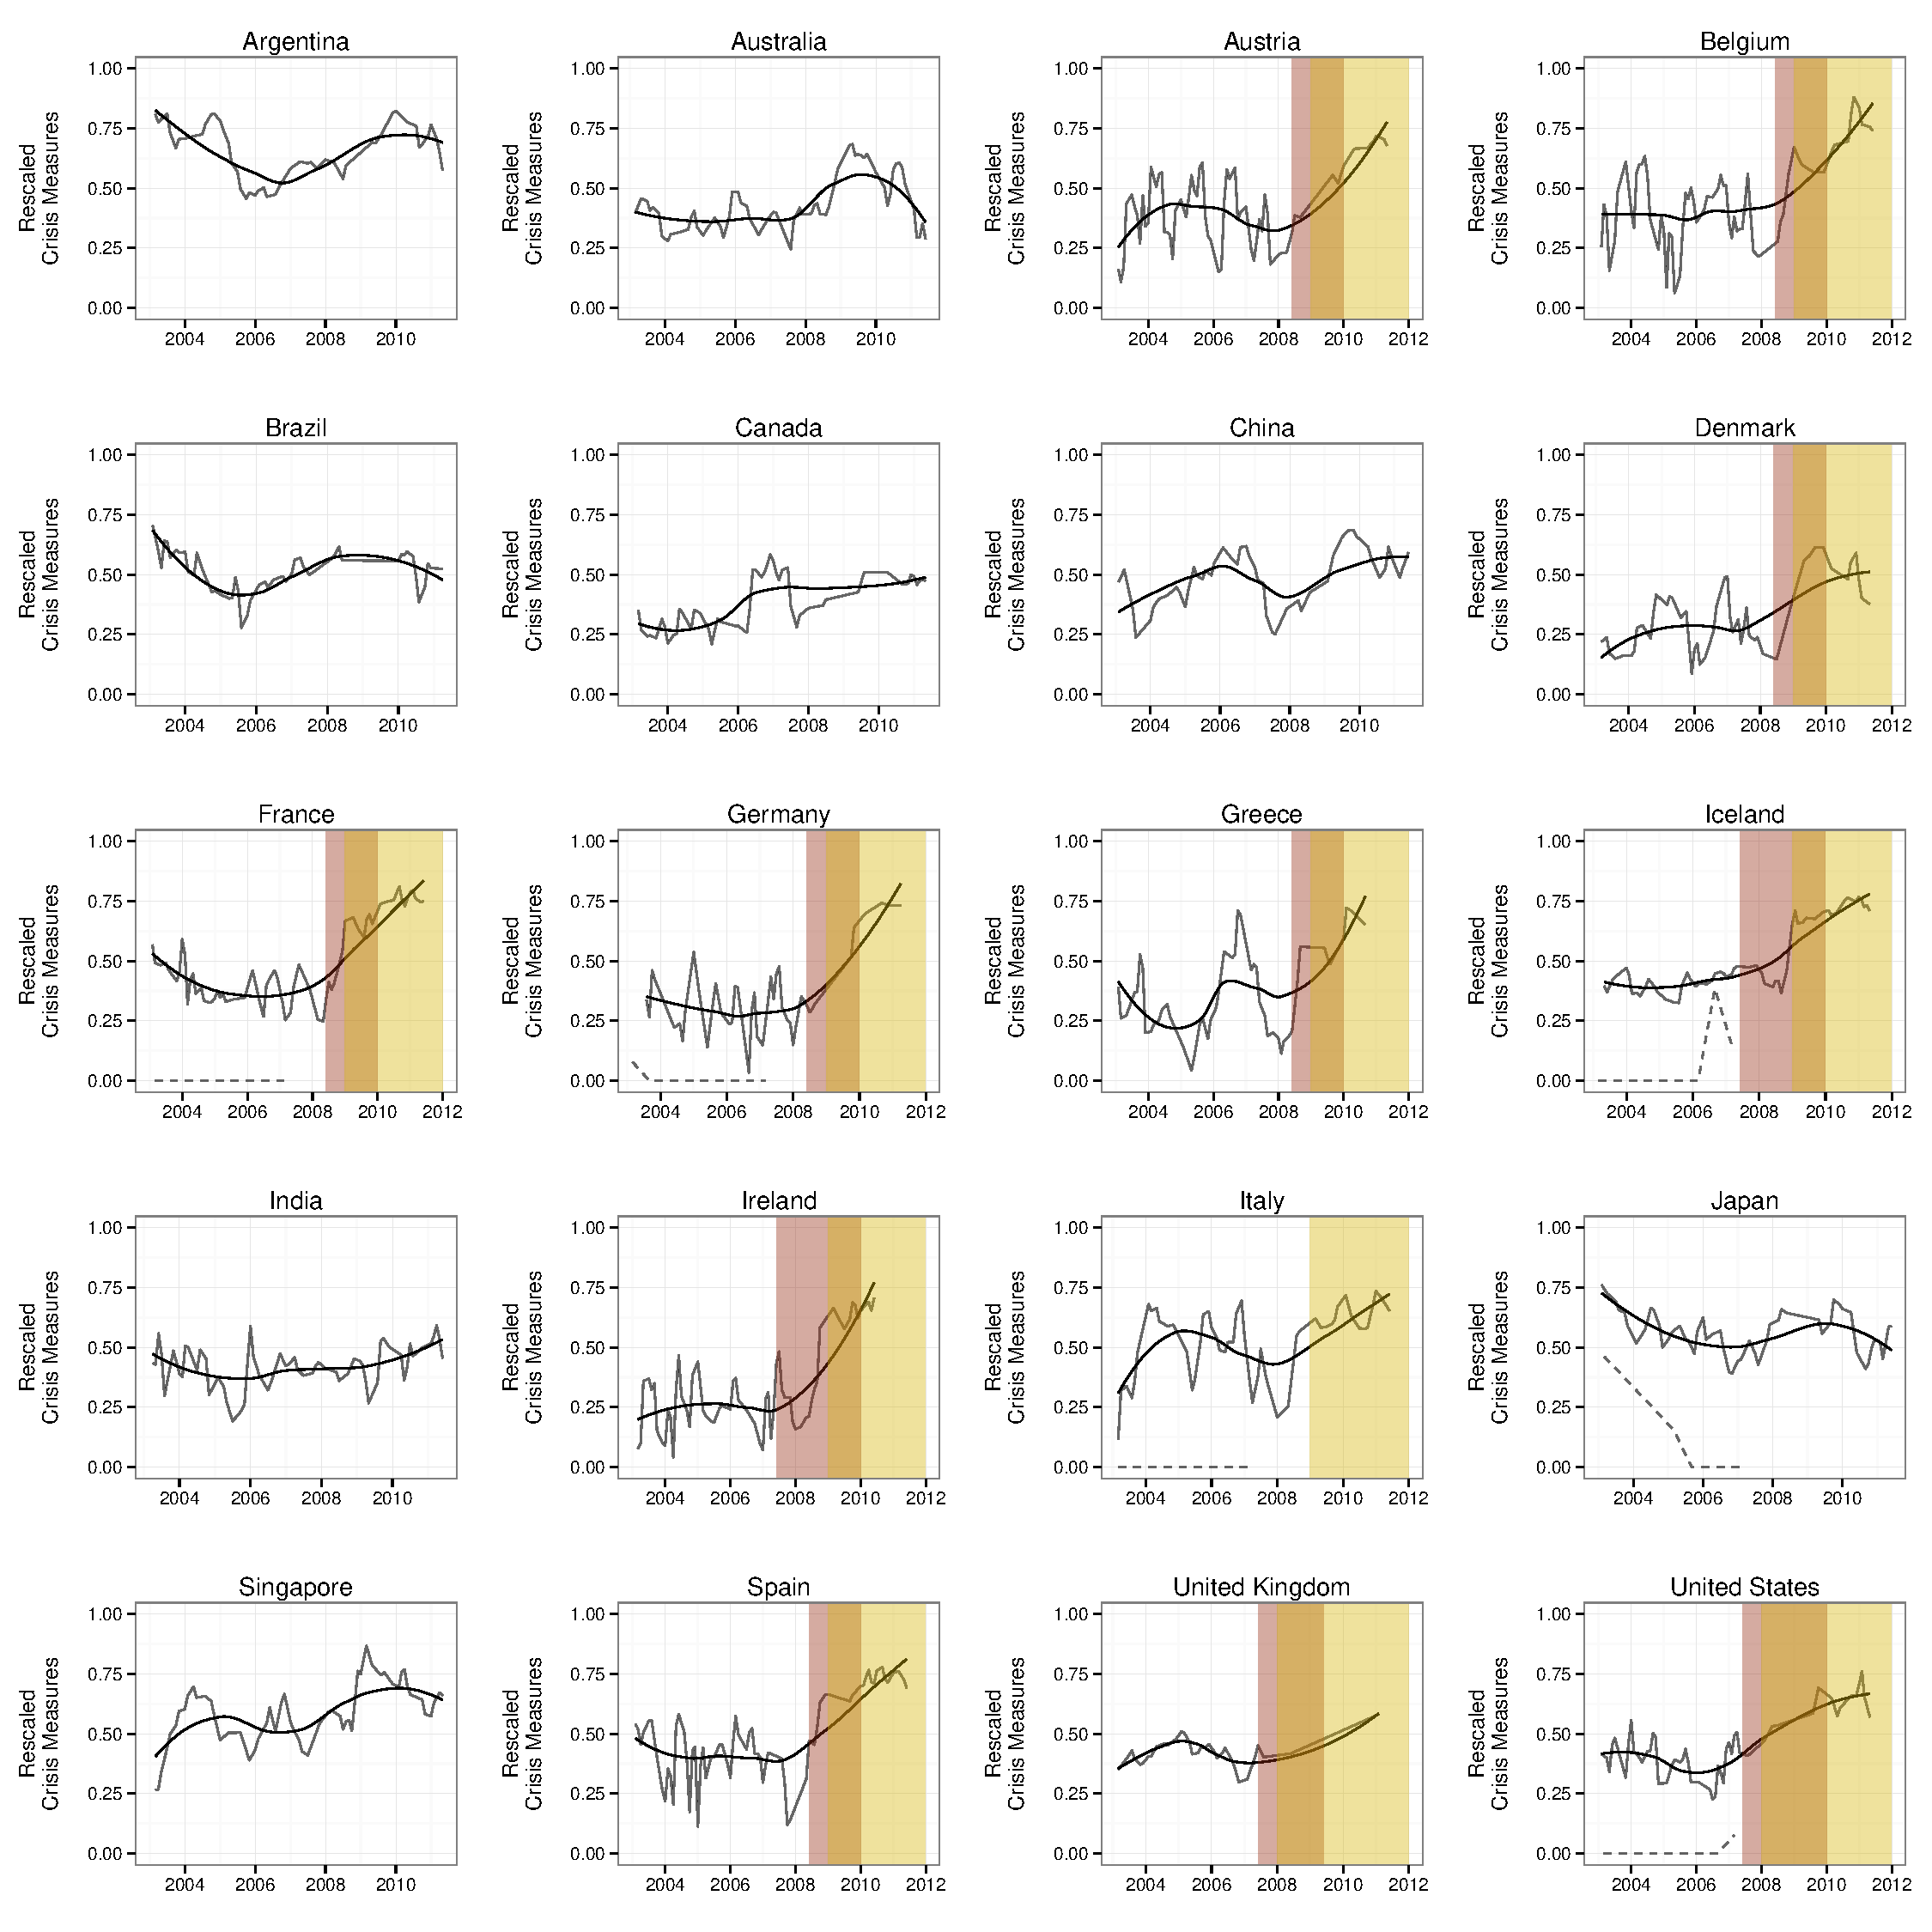
\includegraphics[scale=0.4]{analysis/figures/compare_to_lv_rr.pdf}
    \end{center}

    {\tiny{Solid lines show the (rescaled) EIU Perceptions of Financial Market Stress indicator. Dotted lines represent a loess smooth of these series. \\

    Yellow shaded areas indicate periods that \cite{laeven2013} classify as systemic banking crises. Note that crises are automatically terminated at the end of 2011 due to the series not extending beyond this point, not necessarily because the crisis finished. \\

    Red shaded areas indicate periods that \cite{Reinhart2009} classify as banking crises. Note that crises are automatically terminated at the end of 2009 due to the series not extending beyond this point, not necessarily because the crisis finished. \\

    Orange areas indicate periods where a crisis is recorded for both measures.}}
\end{figure}

\begin{figure}
    \caption{Comparing Perceptions of Financial Market Conditions to \cite{laeven2013} and \cite{Reinhart2009} (2)}
    \label{compare_2}
    \begin{center}
        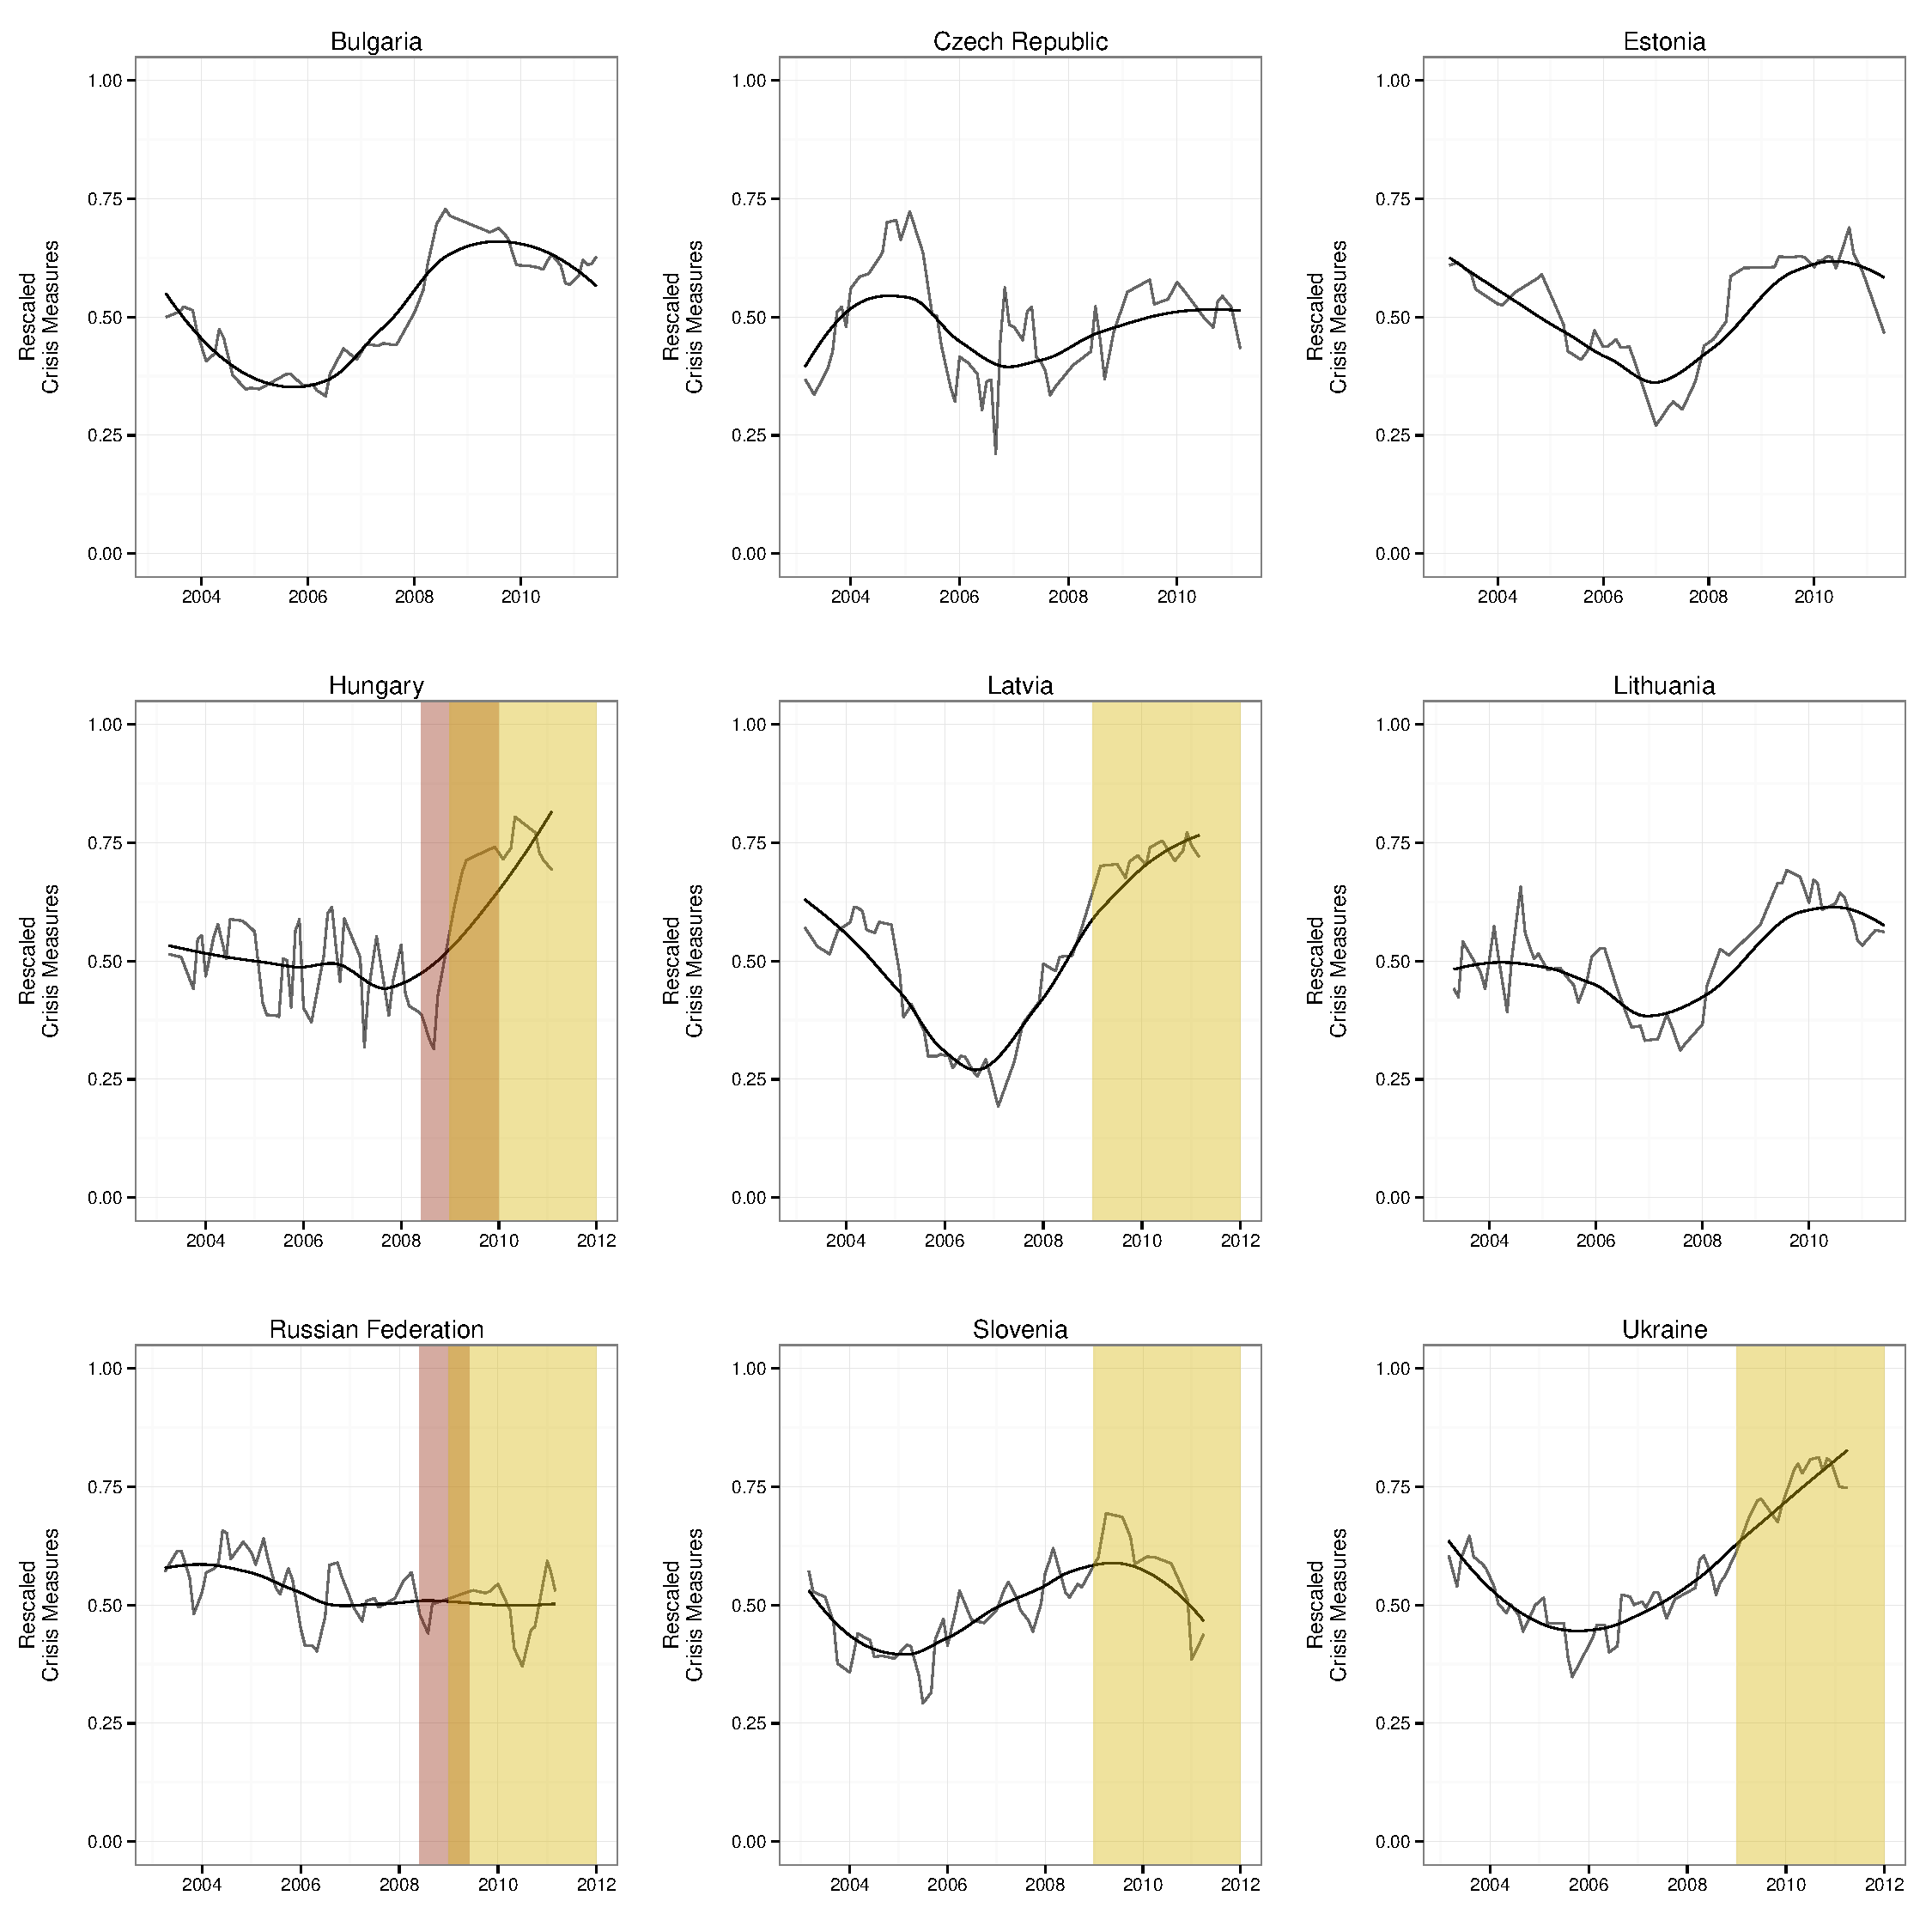
\includegraphics[scale=0.4]{analysis/figures/compare_to_lv_rr_2.pdf}
    \end{center}

    {\tiny{Solid lines show the (rescaled) EIU Perceptions of Financial Market Stress indicator. Dotted lines represent a loess smooth of these series. \\

    Dashed lines show Romer and Romer's \citeyearpar{Romer2015} index rescaled. \\

    Yellow shaded areas indicate periods that \cite{laeven2013} classify as systemic banking crises. Note that crises are automatically terminated at the end of 2011 due to the series not extending beyond this point, not necessarily because the crisis finished. \\

    Red shaded areas indicate periods that \cite{Reinhart2009} classify as banking crises. Note that crises are automatically terminated at the end of 2009 due to the series not extending beyond this point, not necessarily because the crisis finished. \\

    Orange areas indicate periods where a crisis is recorded for both measures.}}
\end{figure}

\subsection{Comparision to Accounting Measures of Banking System Fragility}

How does the EPFMS compare to the widely used Z-Score measure of banking system fragility? Though they measure different quantities--perceptions for the former, bank accounting quantities for the latter--both potentially provide indications of national banking market stress. We might expect them to be related to one another, either being positively correlated and/or one acting as a leading indicator of the other.

We compare the EPFMS to the Bank Z-Score measure compiled from Bankscope data by the World Bank's Global Financial Development Database project \citep{worldbank2013}.\footnote{Indicator ID: GFDD.SI.01. Accessed June 2015.} The measure is interpretable as the inverse of the upper bound of the probability of the banking system's insolvency.\footnote{Formally: $\frac{\mathrm{ROA}_{t} + \frac{\mathrm{equity}_{t}}{\mathrm{assets}_{t}}}{\sigma_{\mathrm{ROA}}}$. $\mathrm{ROA}$ is return on equity. $\sigma_{\mathrm{ROA}}$ is presumably for the entire period for which data is available, though the World Bank's documentation does not explicitly specify this. It is common in other work for the $\sigma_{\mathrm{ROA}}$ to be based on a three year rolling window \cite[225]{beck2013bank}. All quantities are in country aggregates.} Figure~\ref{z_score} shows a comparison of the two measures for selected countries. Note that to ease visual comparability we rescaled the Z-Score to be within zero and one as before, and also reversed the scale so that larger values indicate a higher probability of banking system insolvency.\footnote{It is also common to log-transform the Z-Scores \cite[225]{beck2013bank}. However, it is unclear how this is done as there are negative values in the Z-score that create undefined values when logged.} We also converted the EPFMS to yearly averages for comparability.

There appears to be very little relationship between Z-Scores and the EPFMS Index. The rescaled Z-Score is positively correlated with the EPFMS, as we would expect, but this is very weak with a correlation coefficient of 0.07 (significant at the 5\% level). Interestingly, the Z-Score does not vary significantly within countries over time, especially compared to the EPFMS. There is very little difference between Z-Scores for countries during the financial crisis (however measured) and during more stable times. Thus Z-Scores may not be useful indicators of financial crisis. Z-Scores also do not appear to predict perceptions of financial market stress. In a simple dynamic linear regression that had EPFMS as the dependent variable and included lagged EPFMS, lagged Z-Scores, and country fixed-effects, Z-Scores were not statistically significantly associated with perceptions of financial market stress. It is beyond the scope of our article to determine why the Z-Score is a sub-optimal measure of financial market stress. However, the measure's peculiar aspects found here are important to note for future researchers: the indicator has weak time-variance, it does not distinguish between periods of significant know financial market stress and less stressful times, and it has poor power predicting perceived financial market stress.

\begin{landscape}
\begin{figure}

    \caption{Annual Mean EPFMS Compared to Country-level Z-Scores}
    \label{z_score}

    \begin{center}
        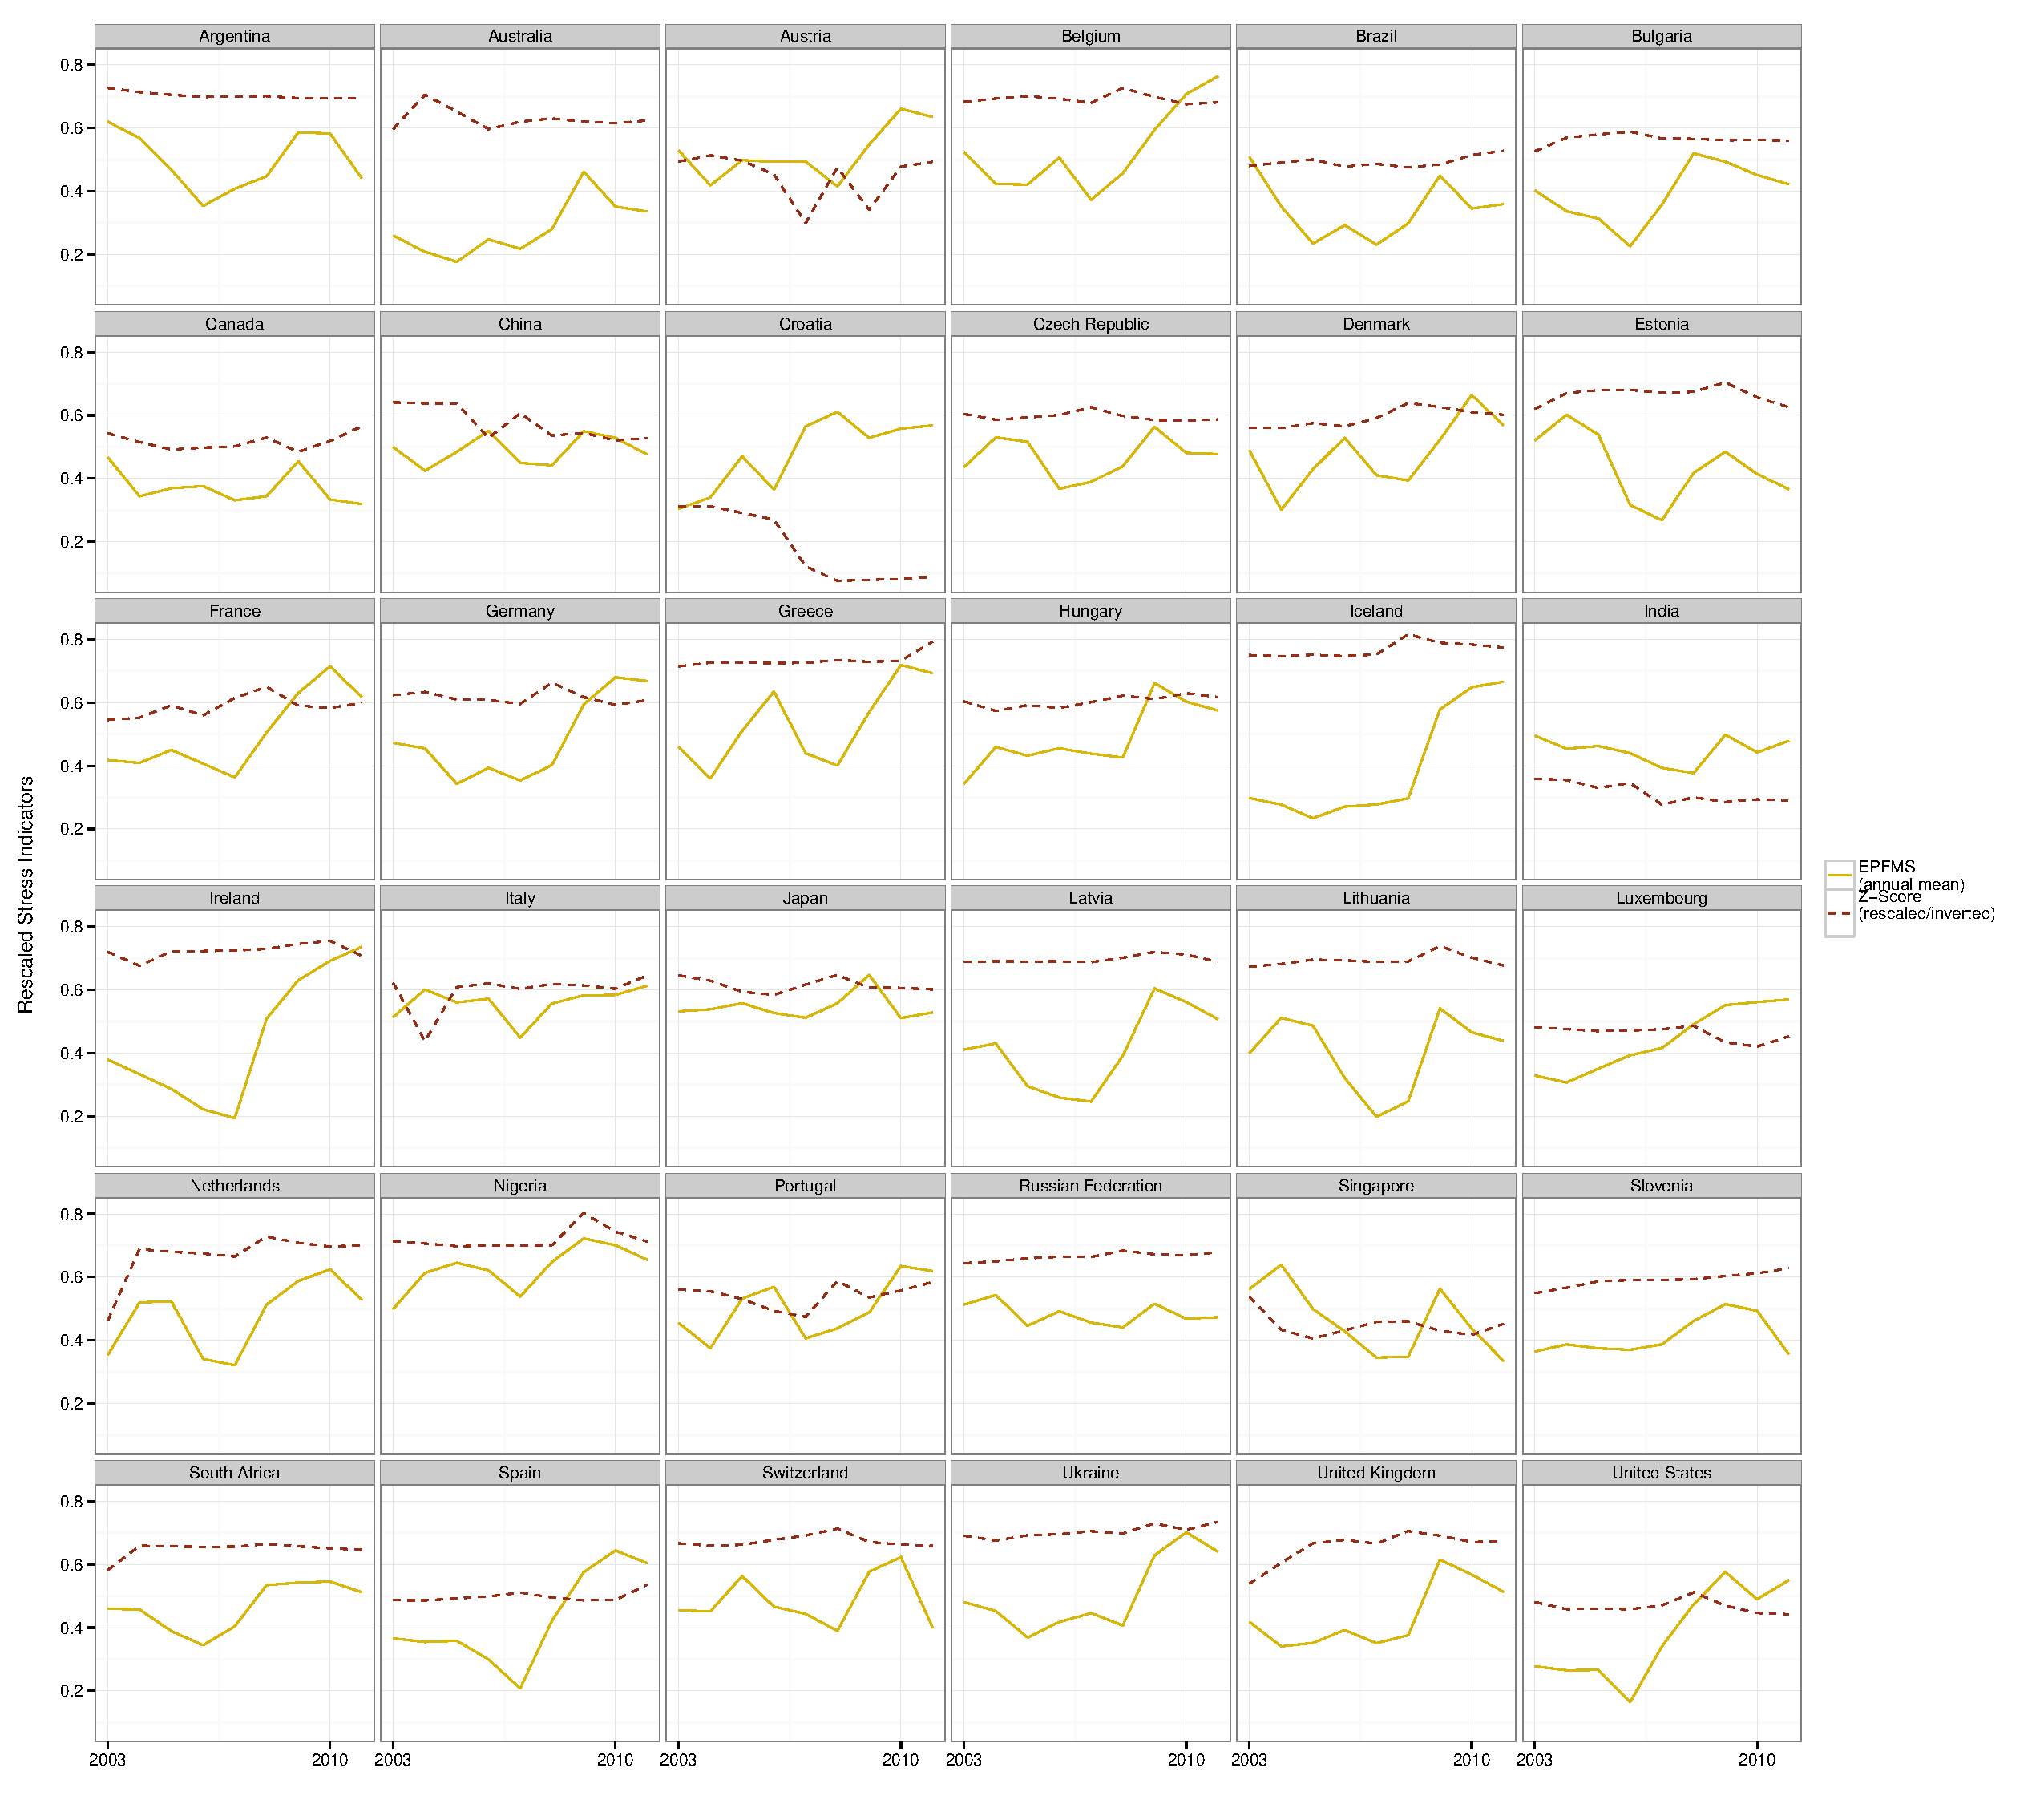
\includegraphics[scale=0.4]{analysis/figures/compare_to_z-score.pdf}
    \end{center}

\end{figure}
\end{landscape}

\subsection{Developed vs.~Developing
countries}\label{developed-vs.developing-countries}

An important finding from examining the Index is that there is a clear
difference in the level of perceived financial market stress in
developed and developing countries. Notably, developing countries often
have scores well above 0.5, while many developed countries only reach
this level during financial crises. Developing countries often lack
strong financial institutions and systems {[}CITE{]}, so we should
expect them to face generally tighter credit market conditions than
developed countries. Formal financial markets are less important for
developing countries' economies {[}CITE{]}.

These observations should lead to an important refinement to how the
Index should be interpreted and how it should be used in empirical work.
First, the Index measures banking market conditions, but not ``crisis''
directly. Instead, perceived crisis is likely the result of an
interaction between the Index and the importance of financial markets
for sustaining a country's economy. Though policy-makers in developing
economies face generally tight credit market conditions, these
persistent conditions likely do not threaten the wider \emph{status quo}
economy. As such, we would not expect significant policy responses to
address financial market stress in these places. Conversely, tightening
of credit market conditions in a developed, financialized economy would
likely have large negative implications for the wider economy. So, we
would expect these politicians to respond to worsening credit market
conditions.

Previous measures of financial market distress and crises have generally
been unable to explore this possible interaction. \emph{Post-hoc}
measures of crisis in particular capture the outcome of this process,
rather than the process itself.

\section{Summarizing Changes in the EPFMS}

So far we have largely examined EPFMS score \emph{levels}. Now we turn to examining \emph{changes} in the EPFMS. To do this we use nonparametric drift-diffusion-jump models (DDJ) \citep{Carpenter2011,Dakos2012}. This approach allows us to draw more general conclusions about how perceptions of financial market stress change in more demanding and less demanding times.

This approach allow us to approximate processes of change in a time series without needing to make explicit assumptions about the underlying process that creates these changes.\footnote{It should be stressed that unlike in other applications of DDJ models, such as in ecology and related work in finance \citep{Kou2008}, that use them to predict future states, we are exclusively using this statistical approach to summarize changes and elucidate patterns in observed data.}

Drift is a measure of local rate of change. Diffusion is the small changes that happen at each time increment. Jumps are larger shocks that occur intermittently and are uncorrelated in time.

The approach we take to estimating the DDJ model is from \cite{Carpenter2011}. It approximates the unknown process generating the EPFMS scores:

\begin{equation}
      dx_{t} = f(x_{t},\;\theta_{t})dt + g(x_{t},\;\theta_{t})dw + dJ_{t}
\end{equation}

\noindent $dx_{t}$ is the change in the EPFMS score $x$ for a country at time $t$. $\theta_{t}$ is a critical transition parameter. The drift function is given by $f(x_{t}\theta_{t})dt$. The diffusion function is given by $g(x_{t}\theta_{t})dw$. $J$ is a jump process. Please see Dakos et al. \citeyearpar[7]{Dakos2012} for further details.\footnote{We estimated the model using the \texttt{ddjnonparam\_ews} function from the \textbf{earlywarnings} R package \citep{earlywarnings2013}.} Note that we estimated the parameters for each country's time series separately.

In the abstract we would perhaps expect that jumps would be more common in countries' EPFMS scores during crisis periods because there would be large moves in the index. To test this we first graphically compared the distributions of jump and diffusion parameters across what Laeven and Valencia\footnote{They are the most recently updated and comprehensive binary measure of crises.} classify as crisis and non-crisis periods. Figure \ref{comp_jump_diff} shows these densities. We have also included a measure of total variance, which is a summary of both jump and diffusion parameters.

\begin{figure}
    \caption{Diffusion, Jump, and Total Variance Estimate Distributions Across Crisis and Non-Crisis Periods from \cite{laeven2013}}
    \label{comp_jump_diff}
    \begin{center}
        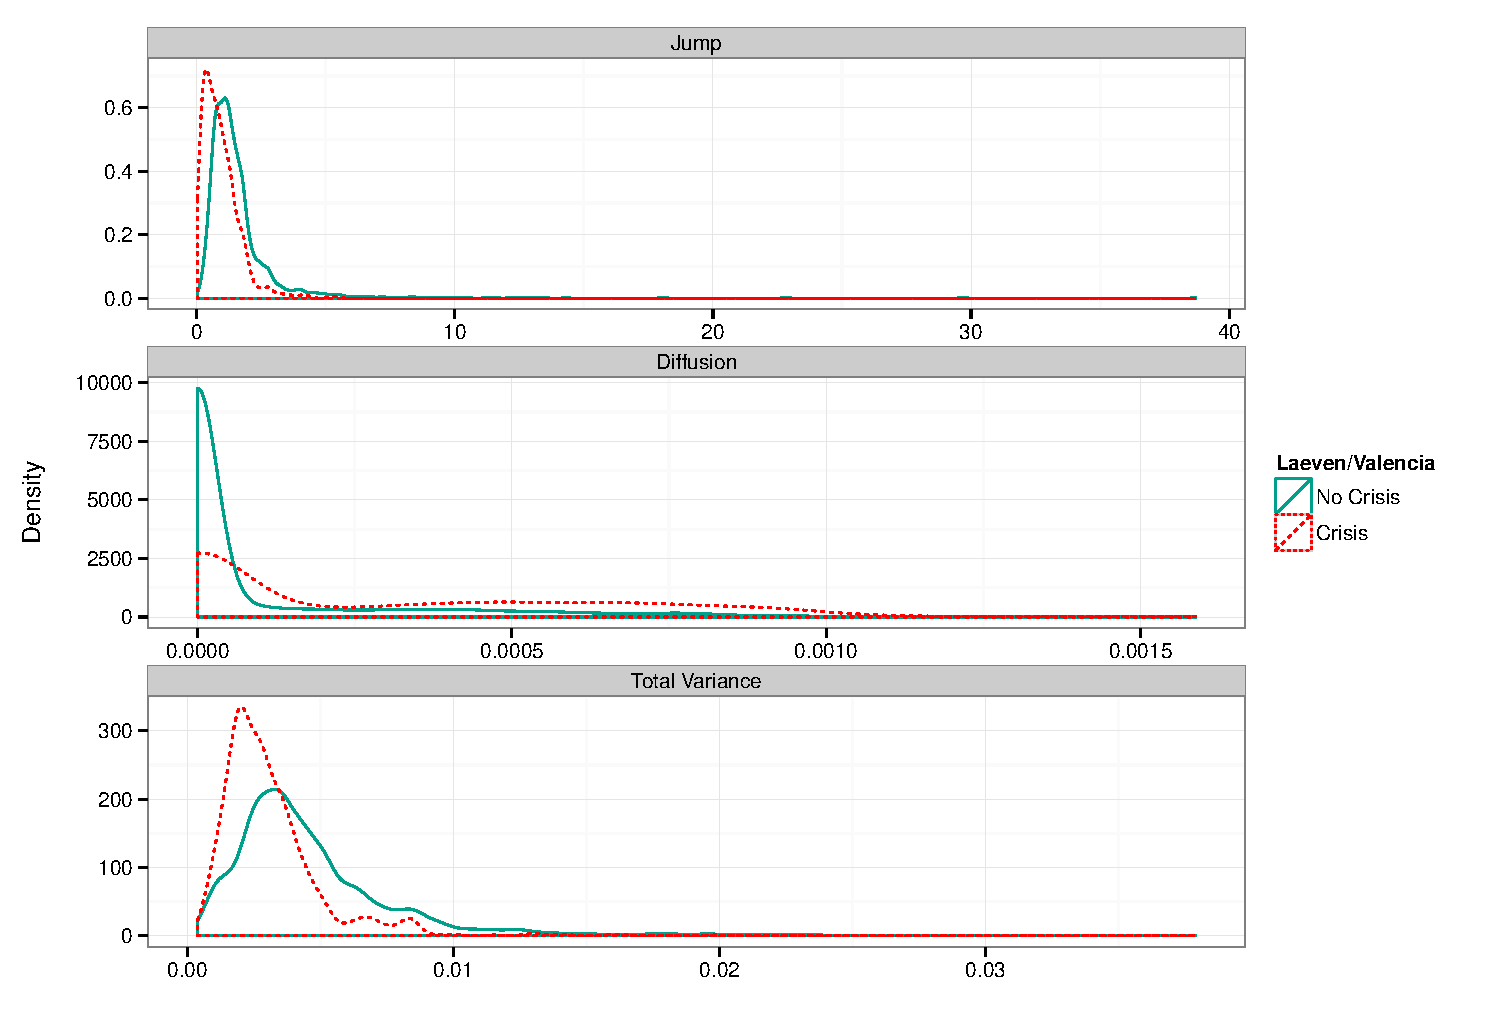
\includegraphics[scale=0.5]{analysis/figures/compare_jump_diffusion_basic.pdf}
    \end{center}
\end{figure}

We can see that the distribution of estimated jump parameters in `non-crisis' periods is shifted upward from the distribution of jump parameters in `crisis' periods. Conversely, the distribution of diffusion parameters in crisis periods is shifted upward from non-crisis periods. Finally, the distribution of total variance in crisis periods is lower than non-crisis periods. We found these distributions to be statistically significantly different in the described direction at all conventional levels using one-sided Kolmogorov–Smirnov tests.\footnote{We ran the tests using the \texttt{ks.test} function from base R.}

This is an interesting result considering our prior expectations. How can we make sense of it? It is useful to refer back to figures \ref{compare_1} and \ref{compare_2}. Notice that many of there periods that are classified across measures as a crisis do indeed begin with a jump. Belgium, Denmark, and Germany are particularly illustrative of this. However, these changes are not unusually large relative to changes in previous years. What is different, however, is what happens after the jump. Before crisis periods there are relatively many jumps in both positive and negative directions. In crisis periods there are a few positive jumps followed by many smallish, often positive, changes in the EPFMS.

In non-crisis times there may effectively be more noise in economic events, causing relatively large positive and negative swings in perceptions of financial market conditions. When crises occur, the information used to create perceptions of financial market stress are clearer. Think for example of Lehman Brother's collapse and the continually bad news that followed. During a crisis initial shocks are followed by additional bad news. During non-crisis times a possible shock could be followed relatively quickly afterwards by good news.

Not all crises are the same. Most of the crises in the period for which we have data have been protracted. In some cases, however, crises came quickly and left almost as quickly. Kazakstan is a notable example. In late 2009 there was a prominent spike in perceptions of financial market stress. Within a few months, the EPFMS score returned to almost its previous--though still relatively elevated--trend level.

While the EPMFS is a fine-grained description of perceived stress, we should avoid using it as a predictive measure of when a crisis will begin or end.

\section{Replication}\label{replication}

\section{Conclusions}\label{conclusions}


\bibliographystyle{apsr}
\bibliography{main.bib}

\clearpage

\section*{Online Appendix}

\todo{Make tables more relevant for paper}

\begin{table}
\caption{Selected Literature Review of Political Institutions and Financial
Crisis (Political Outcomes)}


\label{LitRevTable2}
\begin{center}

\vspace{0.5cm}
\scalebox{0.9}{
\begin{tabular}{ m{2.5cm} m{1.75cm} m{6.25cm} m{2.5cm} }
    \hline
    Work & Crisis Type & Key Arguments/Findings & Crisis Data Sources \\
    \hline\hline

    %%% Bernhard and Leblang
    \cite{Bernhard2008} & Currency crisis & - Changes in the probability that cabinets will collapse condition the probability of speculative attacks.

    - Higher probability of a speculative attack decreases the probability of calling strategic elections. & Own data aggregated from multiple sources \\[0.25cm]\hline

    %%% Chwieroth and Walter
    \cite{Chwieroth2013} & Banking crises &  - Probability of government survival during crises changed over time as expectations changed about what governments should do to respond.

    - Governments with more veto players after the inter-war period are treated more harshly by voters. & \cite{ReinhartRog2010} \\[0.25cm]\hline

    \cite{CrespoTenorio2014} & Banking crisis & - Increasing globalization weakens the accountability link between politicians and voters.

    - Incumbents in open capital economies are more likely to survive a crisis, than those in closed economies. & Own data aggregated from multiple sources. \\[0.25cm]\hline

    %%% Montinola
    \cite{Montinola2003} & Banking crisis & - IMF credits decrease the probability of resolving banking crises.

    - The decisiveness of a political regime significantly influences the probability of emerging from systemic distress, though this depends on whether the crisis is moderate or severe. & Own data aggregated from multiple sources \\[0.25cm]\hline

    %%% Pepinsky
    \cite{Pepinsky2012} & Banking crisis & - Two factors--incumbent governments' responsibility for the current crisis and their responsiveness to its domestic economic effects--shape the political effects of the global economic crisis. & \cite{Laeven2010} \\[0.25cm]\hline

    \hline
\end{tabular}

}
\end{center}
\end{table}

\begin{table}[H]
\caption{Selected Literature Review of Political Institutions and Financial
Crisis (Crisis Occurrence, Policy Choices/Policy Outcomes)}


\label{LitRevTable}
\begin{center}

\vspace{0.5cm}
{\tiny{
\begin{tabular}{ m{2.5cm} m{2cm} m{7cm} m{3cm}}
    \hline
    Work & Crisis Type & Key Arguments/Findings & Crisis Data Sources \\
    \hline\hline

    %%% Broz
    \cite{broz2013} & Banking crisis & - In OECD countries right-wing governments pursue policies that lead to financial instability. Voters respond to resulting crises by voting in left-wing governments. & \cite{Reinhart2009,Laeven2012} \\[0.25cm]\hline

    %%% Galasso
    \cite{galasso2014} & Financial and economic crises & - Governments respond to financial crises by increasing regulation. & Dummy based on OECD output gap below -3.4\% \\[0.25cm]\hline

    %%% Gandrud
    \cite{Gandrud2013,Gandrud2014} & Banking crises & - Best practice financial governance institutional designs are more likely to be adopted during crises when there is high uncertainty about policy choices and outcomes. & \cite{Laeven2008,ReinhartRog2010} \\[0.25cm]\hline

    %%% Ha and Kang
    \cite{ha2015} & - Banking crisis & Developing countries respond to crises with fiscal and monetary tightening, which was moderated by political constraints, left ideology governing parties, and up coming elections. & \cite{Laeven2008}. \\[0.25cm]\hline

    %%% Hallerberg Scart
    \cite{HallerbergScartForthcoming} & Banking, debt crises & - Banking crises reduce the probability of fiscal reforms, but the longer a crisis lasts and if it becomes a sovereign debt crisis the the probability of reform increases.

    - Countries with more personalistic voting are more likely to reform. & \cite{Laeven2012} for Latin American countries \\[0.25cm]\hline

    %%% Hallerberg Wehner
    \cite{Hallerberg2013} & Banking, currency, debt crises & - Some evidence that more technically competent ministers of finance are appointed during debt crises. Not much robust evidence for other effects of crisis on the technical competency of economic policy-makers. & \cite{Laeven2012}  \\[0.25cm]\hline

    %%% Hicken et al.
    \cite{Hicken2005} (2005) & Growth shocks & - The size of the winning coalition is positively associated with growth recoveries following forced devaluations. & Own data aggregated from multiple sources \\[0.25cm]\hline

    %%%% Keefer
    \cite{Keefer2007} & Banking crises & - Higher electoral competitiveness leads to faster and less costly crisis responses.

    - Checks and balances not associated with crisis policy choices or outcomes. & Modified \cite{Honohan2003} \\[0.25cm]\hline

    %%% Kleibl
    \cite{Kleibl2013} & Banking crisis & - Responses to regulatory failures are conditioned by the level of public ownership in the banking sector. & \cite{Laeven2010,Reinhart2009} for OECD countries \\[0.25cm]\hline

    %%% MacIntyre
    \cite{MacIntyre2001} & Financial crises & - U-shaped relationship between veto players and crisis outcomes & Own data aggregated from multiple sources \\[0.25cm]\hline

    %%% Reischmann
    \cite{reischmann2015} & Banking crises & - Creative accounting as measured by changes in the stock flow adjustment occurs more during financial crises, though effect may be swallowed up by the period fixed effects in his regressions as crises are highly correlated with time in his sample. & \cite{Laeven2012} \\[0.25cm]\hline

    %%% Rodrick
    \cite{Rodrick1999} & Growth shock & - Many veto players, if organized to manage conflicts, will result in more appropriate and quickly implemented crisis management policies. & Own data aggregated from multiple sources \\[0.25cm]\hline

    %%%% Rosas
    \cite{Rosas2006,Rosas2009} & Banking crisis & - Democratic regimes have fewer bailouts.

    - Central bank independence and transparency lead to fewer bailouts. & Modified \cite{Honohan2000} \\[0.25cm]\hline

    %%% Seiferling and Tareq
    \cite{seiferling2015} & Banking crisis & - Find advanced economies governments extend more loans and purchase more equities in temporarily insolvent firms during financial crisis than emerging market governments. & \cite{Laeven2010} via \cite{weber2012} \\[0.25cm]\hline

    %%% Satyanath
    \cite{Satayanath2006} & Banking crises & - Executives without `banking cronies' and that are not prevented from appointing their own bureaucrats by many veto players are more likely to have stringent financial regulation that prevents crises. & Case studies of 7 East Asian countries using own data \\[0.25cm]\hline

    %%% Wibbels and Roberts
    \cite{Wibbels2010} & Currency, growth, \& fiscal crises & - Unions and strong left parties are more associated with crises, though combined strong unions-left parties may alleviate inflationary crises. & Own data aggregated from multiple sources for 17 Latin American countries \\[0.25cm]\hline


    \hline
\end{tabular}

}}
\end{center}
\end{table}





\end{document}
